\chapter{Arquitectura Implementada} \label{cap:seis}

La arquitectura implementada tiene como finalidad que el sistema web que se desarrolle sea estable, modular y escalable; En la Figura \ref{fig:arqui} se ilustra el diagrama  detalladamente junto con sus componentes.

\begin{figure}[H]
	\begin{center}
		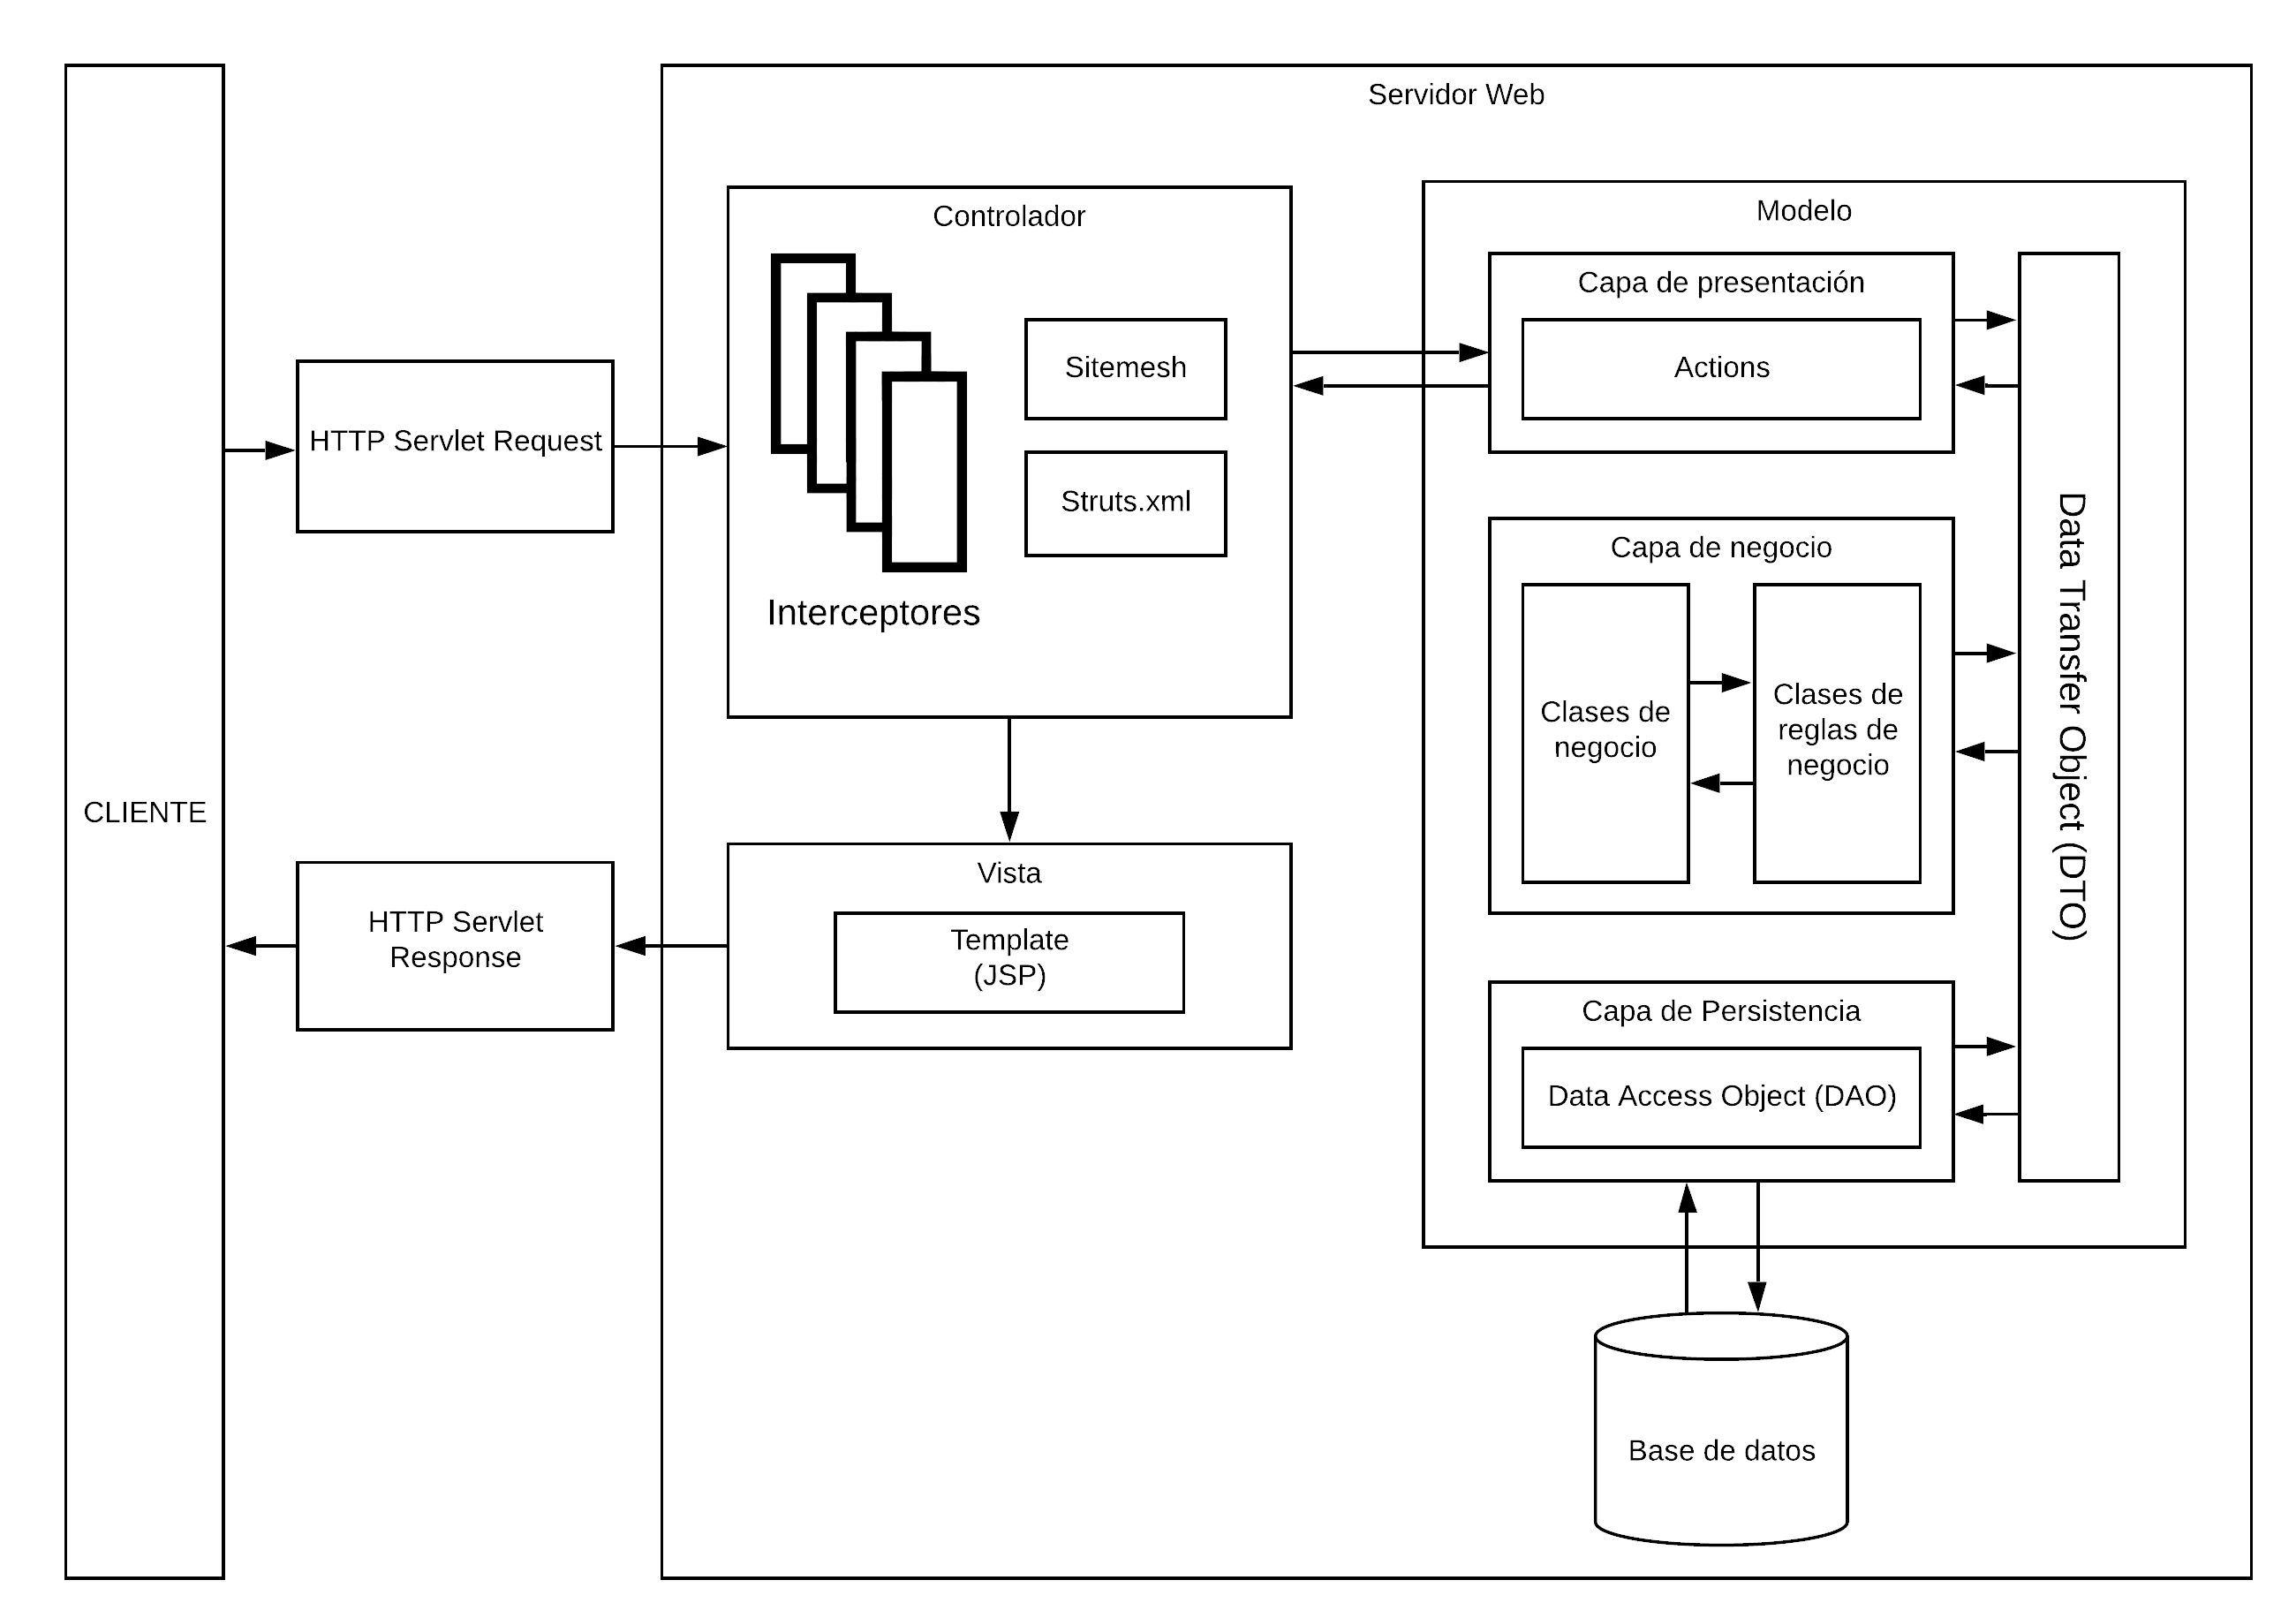
\includegraphics[width=.75\textwidth]{images/arquitectura/DiagramaArquitecturaTesseract}
		\caption{Arquitectura implementada}
		\label{fig:arqui}
	\end{center}
\end{figure}

La arquitectura esta compuesta de esta manera ya que se acopla perfectamente a la estructura definida, la arquitectura principal es Cliente-Servidor donde el cliente se comunica con el servidor por medio de internet a través de peticiones con el Protocolo de Transferencia de Hipertexto (Hypertext Transfer Protocol, HTTP por sus siglas en ingles) Servlet Request recibiendo una respuesta HTTP Servlet Response.\\

El servidor implementa el patrón de diseño MVC a través del Framework Struts 2 teniendo la siguiente estructura:
\begin{itemize}
	\item Modelo: La capa Modelo es la encargada de realizar el procesamiento de los datos obtenidos del cliente, el modelo debe aplicar las reglas de negocio y realizar las operaciones correspondientes en la base de datos.
	
	\begin{itemize}
	
	\item Dentro de la capa de modelo se implementó una arquitectura de N capas, donde: la capa de presentación contiene los Actions; la capa de negocio contiene las clases de negocio y las clases de reglas de negocio; la capa de persistencia contiene las clases de acceso a datos (Data Access Objects, DAO’s por sus siglas en inglés).\\
	
	\item La transferencia de datos entre las capas se realizó mediante clases de transferencia de datos (Data Transfer Object,  DTO’s por sus siglas en inglés).
	
	\end{itemize}
	
	\item Controlador: La capa controlador es la encargada de recibir la petición del cliente, aplica los interceptores declarados y mediante el archivo de configuración (struts.xml) redirige al action correspondiente, cuando el modelo regresa una respuesta, el archivo de configuración sabe que las Páginas de Servidor Java (JavaServer Pages, JSP por sus siglas en inglés) deben renderizar comunicándose con la capa de vista.
	
	\item Vista: La capa vista es la encargada de renderizar el JSP correspondiente y enviar la respuesta al cliente que la solicitó.
\end{itemize}


\section{Modelo MVC}
El patrón de diseño MVC es fundamental para la separación entre lógica de interfaz de usuario y lógica de negocio \hyperlink{b30}{[30]}; de esta manera la estructura del proyecto tiene las siguientes características \hyperlink{b31}{[31]}:

\begin{itemize}
	\item Los objetos del modelo de datos encapsulan información.
	\item Los objetos de vista muestran información al usuario.
	\item Los objetos del controlador implementan acciones.
	\item Los objetos de vista observan los objetos del modelo de datos y actualizan su \item visualización cada vez que cambian los objetos del modelo.
	\item Los objetos de vista recopilan la entrada del usuario y la pasan a un objeto controlador que realiza la acción. 
\end{itemize}

Para su realización se utilizaron las siguientes tecnologías:

\section{Arquitectura N Capas}
La arquitectura n capas está implementada dentro del patrón MVC en el Modelo, ayuda a la modularidad de la capa de negocio, la capa de reglas de negocio y la capa de persistencia, de tal manera que se consigue un bajo acoplamiento.

\section{Patrones de Diseño}

\subsection{Singleton}
El patrón de diseño singleton se implementó mediante anotaciones de Spring, cuando un bean es anotado con el alcance Singleton, solo se administrará una instancia compartida del bean, y todas las solicitudes de beans con un id o ids que coincidan con esa definición de bean harán que el contenedor Spring devuelva una instancia de bean específica \hyperlink{b28}{[28]}, de esta manera se convierte en un objeto administrado por Spring.\\

La ventaja de esta arquitectura es la capacidad de adaptación, si en algún momento se debe modificar alguna capa, por ejemplo la capa de persistencia, ésta modificación no afectaría a las otras capas ya que la comunicación entre ellas es transparente.

\subsection{Factory}
El patrón de diseño Abstract Factory lo utilizamos cuando configuramos la clase StrutsSpringObjectFactory, que extiende de objectFactory, y se delega la responsabilidad de creación de objetos a Spring, de esta manera este patrón encapsula un grupo de fábricas, cada objeto fuera del cual actúa como una fábrica independiente.

\subsection{Facade (Fachada)}
El patrón de diseño facade proporciona interfaces comunes a las clases de sistema y facilita la separación de tareas, de esta manera se oculta la complejidad. Se implementó en la capa de negocio, ya que para obtener o enviar información a esta capa solo se debe llamar un método. 

\subsection{Adapter (Adaptador)}
El patrón de diseño Adapter se utiliza a través de Struts en los archivos de propiedades, provee un wrapper para la internacionalización.

\subsection{Data Access Object (DAO)}
El patrón de diseño DAO se utiliza para abstraer y encapsular todo el acceso a la fuente de datos. El DAO gestiona la conexión con la fuente de datos para obtener y almacenar datos . Se crearon DAO’s genéricos y específicos además de NamedQueries para su utilización en este patrón.

\subsection{Data Transfer Object (DTO)}
El patrón de diseño DTO se utiliza para encapsular los datos de negocio. Se utilizó este patrón de diseño para transferir los datos entre la capa de presentación, la capa de negocio y la capa de persistencia, de tal manera que los DTO’s no tengan objetos de tipo Entity.

\subsection{Decorator}
El patrón de diseño Decorator agrega funcionalidad a los objetos; un objeto Decorator "envuelve" un Componente, es decir, todos los clientes del Componente hacen referencia al Decorador envolvente en lugar de directamente al Componente. Se utilizó este patrón al incluir Sitemesh para Struts2, de esta manera al mostrar las vistas (JSP) todas incluirán los menús correspondientes.\\

La ventaja de esta arquitectura es la capacidad de adaptación, si en algún momento se debe modificar alguna capa, por ejemplo la capa de persistencia, ésta modificación no afectaría a las otras capas ya que la comunicación entre ellas es transparente.
